\section{Da Mixed Side Information a Wyner-Ziv}
\label{sec:msi-system-to-wz}

\begin{prop}
    \label{prop:msi-to-wz}

    Sia \(X\) la sorgente codificata da un sistema Mixed Side Information
    \cite{1614094}. Sia \(Y\) l'informazione laterale nota sia al codificatore
    che al decodificatore di questo sistema e \(Z\) l'informazione laterale
    nota al solo decodificatore. Tale sistema può essere ridotto a un sistema
    Wyner-Ziv \cite{1055508} dove la sorgente è \(X'=X,Y\) e l'informazione
    laterale (nota al solo decodificatore) è \(Z'=Y,Z\).
\end{prop}

\begin{figure}[hb]
    \centering
    \begin{subfigure}[b]{0.45\textwidth}
        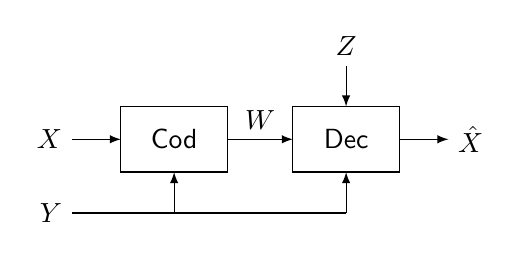
\begin{tikzpicture}[scale=0.52,>=latex]
    \tikzstyle{every node}=[font=\fontsize{10}{12}\sffamily]

    \draw[->] (0,0.8) node[left]{\(X\)} -- (1.2,0.8);

    \draw (1.2,0) rectangle (3.8,1.6)
    node[midway,align=center]{Cod};

    \draw[->] (3.8,0.8) -- (5.4,0.8)
    node[above,midway]{\(W\)};

    \draw (5.4,0) rectangle (8,1.6)
    node[midway,align=center]{Dec};

    \draw[->] (8,0.8) -- (9.2,0.8)
    node[right]{\(\hat{X}\)};

    \draw[<-] (6.7,1.6) -- (6.7,2.6)
    node[above]{\(Z\)};

    \draw[-] (0,-1) node[left]{\(Y\)} -- (6.7,-1);
    \draw[->] (2.5,-1) -- (2.5,0);
    \draw[->] (6.7,-1) -- (6.7,0);
\end{tikzpicture}

        \caption{}
        \label{fig:mini-msi}
    \end{subfigure}
    \begin{subfigure}[b]{0.54\textwidth}
        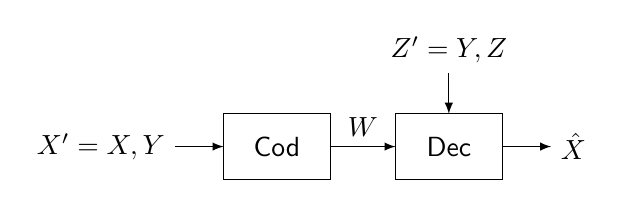
\begin{tikzpicture}[scale=0.52,>=latex]
    \tikzstyle{every node}=[font=\fontsize{10}{12}\sffamily]

    \draw[->] (0,0.8) node[left]{\(X'=X,Y\)} -- (1.2,0.8);

    \draw (1.2,0) rectangle (3.8,1.6)
    node[midway,align=center]{Cod};

    \draw[->] (3.8,0.8) -- (5.4,0.8)
    node[above,midway]{\(W\)};

    \draw (5.4,0) rectangle (8,1.6)
    node[midway,align=center]{Dec};

    \draw[->] (8,0.8) -- (9.2,0.8)
    node[right]{\(\hat{X}\)};

    \draw[<-] (6.7,1.6) -- (6.7,2.6)
    node[above]{\(Z'=Y,Z\)};
\end{tikzpicture}

        \caption{}
        \label{fig:mini-wz}
    \end{subfigure}
    \caption{
        (a) Il sistema Mixed Side Information.
        (b) Il sistema Wyner-Ziv.
    }
    \label{fig:mini-schemes}
\end{figure}

\begin{proof}
    È sufficiente mostrare che il tasso di trasmissione in funzione della
    distorsione per un sistema Wyner-Ziv con le caratteristiche descritte dalla
    proposizione (rappresentato in Figura~\ref{fig:mini-wz}) è equivalente al
    tasso di trasmissione in funzione della distorsione di un sistema
    \textit{Mixed Side Information} (\textit{MSI}), mostrato in
    Figura~\ref{fig:mini-msi}. Inoltre, poiché in entrambi i casi il tasso di
    trasmissione è l'estremo inferiore di una certa informazione mutua, è
    sufficiente mostrare che le due informazioni mutue si equivalgono.

    Sia \(W\) la variabile aleatoria ausiliaria per entrambi i sistemi. Per un
    sistema MSI si ha
    \begin{equation}
        \begin{aligned}
            \mutual{X}{W \given Y,Z} &= \mutual{X}{W,Y,Z} - \mutual{X}{Y,Z} \\
            &= \entropy{X} - \entropy{X \given W,Y,Z} - \entropy{X} + \entropy{X \given Y,Z} \\
            &= \entropy{X \given Y,Z} - \entropy{X \given W,Y,Z} \,,
        \end{aligned}
    \end{equation}
    e per un sistema Wyner-Ziv si ha
    \begin{equation}
        \begin{aligned}
            \mutual{X'}{W \given Z'} &= \mutual{X,Y}{W \given Y,Z} \\
            &= \mutual{X,Y}{W,Y,Z} - \mutual{X,Y}{Y,Z}\\
            &= \entropy{X,Y} - \entropy{X,Y \given W,Y,Z} - \entropy{X,Y} + \entropy{X,Y \given Y,Z} \\
            &= \entropy{X,Y \given Y,Z} - \entropy{X,Y \given W,Y,Z} \\
            &= \entropy{X \given Y,Z} - \entropy{X \given W,Y,Z} \,.
        \end{aligned}
    \end{equation}
    Si ha quindi che \(\mutual{X}{W \given Y,Z} = \mutual{X'}{W \given Z'}\) e
    la dimostrazione è conclusa.
\end{proof}
